\section{Background Research \& Analysis}

\subsection{Market Research \& Analysis}
This section details the market research analysed for Opticaff.
The Coffee market was researched as were the different mobile development platforms; which were analysed to determine the most suitable one to use for this prototype application. 
Finally the potential competitors to Opticaff were detailed and analysed to see if any of them pose a genuine threat against it. 

\subsubsection{Coffee Research \& Analysis}
Coffee consumption in the United Kingdom has steadily increased over the past decade. 
In particular the past five years been seen an explosive increase, there are several theories as to why this is the case.
Firstly, instant coffee shops have become more common on our high streets. 
Companies such as Starbucks\texttrademark and Costa\texttrademark have been opening more stores as more citizens have been buying instant coffee; this doesn’t show any signs of slowing down either as Starbucks have recently announced 300 new stores to be opened over the next five years \cite{starbucks}.

Secondly, these brands have contributed to the newfound ‘coolness’ that is associated with coffee \cite{popular}. 
Lastly, there is evidence that the economic climate has played a part in coffee’s rise. 
Also known as the ‘lipstick effect’, Britons have been unable to afford expensive treats for themselves so they have been spending on cheaper treats, a good example of which is coffee \cite{costa}.
This research is important to OptiCaff because it shows that the coffee industry is on the rise, and it would not make business sense for us to invest in a declining industry.

\begin{center}
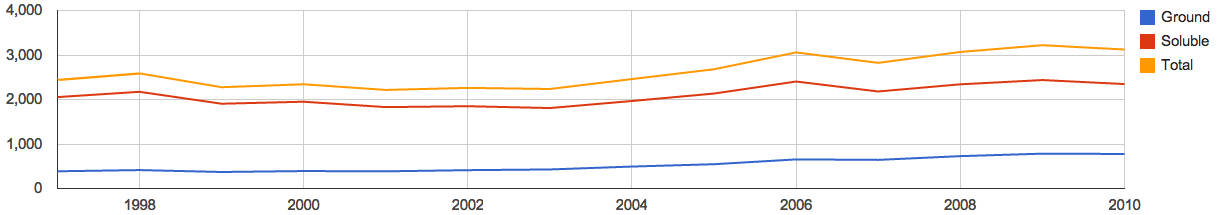
\includegraphics[trim = 0mm 0mm 0mm 0mm, clip, scale=0.38]{images/CaffeineGraph.png}
\end{center}

\subsubsection{Mobile Platform Research}
OptiCaff ’s purpose lent itself heavily to being a mobile application, and as such that sparked the debate of what platform it should be developed for. 
There are various mobile operating systems that Opticaff could be deployed on:

\begin{itemize}
	\item{Google's Android}
	\item{Apple's iOS}
	\item{Blackberry's RIM}
	\item{Windows 7}
\end{itemize}

Based on the Smartphone Operating System statistics from June 2011 Android and Apple are dominating the market at present:

\include{figure}
\begin{center}
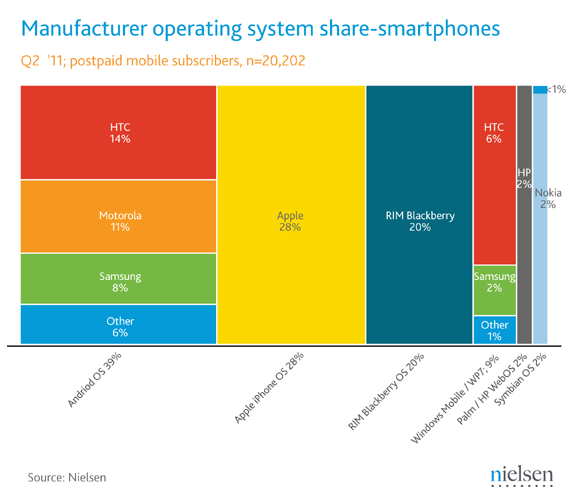
\includegraphics[trim = 0mm 0mm 0mm 0mm, clip, scale=0.38]{images/smartphone.png}
\caption{Manafacture Operating system share-smartphones June 2011 \cite{smartphone}}
\end{center}
\end{figure}


It was decided that for the prototype application, Android \cite{Android} would be the simpler option for the following reasons:
Android can be developed on any platform \cite{SDKAllOS}, which is useful as the group uses a combination of OSX, Linux and Windows.
Android uses Java, which all members of the group have had significant experience with, and given the timescale in which to complete the application, in addition to other commitments it seemed the most viable option. 

There are various mobile operating systems that OptiCaff could be deployed upon. The Android operating system created by Google requires applications to be written in Java which is a positive for the OptiCaff team, all members have Java development experience with one member having Android development experience. Using Android also means no special hardware is required to develop an application, the Android SDK is freely available and IDE’s are also free, Eclipse being an example of this \cite{Eclipse}. The app store for Android phones, Google Play, is a large marketplace that would give OptiCaff a great enough set of potential users.

``Google’s 10 Billion Android App Downloads: By the Numbers" \newline
A negative of Android is the result of it being open-source, manufacturers are able to create a separate version of Android just for their hardware, this means there are now lots of iterations of Android. Developing an application for all these different versions is difficult and OptiCaff would not be compatible with all phones at first.

iOS is the Apple iPhone’s operating system, it requires applications to be written in Objective C, no members in the OptiCaff team have any experience with Objective C. The only IDE available for developing iPhone applications is Xcode which is only available to OS X users, in other words, development is only possible on Apple computers, this is a requirement that is particularly limiting for a small development team. The Apple app store is currently the largest marketplace for mobile applications, although it is slightly ahead of Google Play. Finally, there is only one iteration of iOS, it is not licensed to other companies, the only complication is that there are a few versions running concurrently. This means that an app developed for the iPhone would likely work on all iPhones.

OptiCaff will be developed in Android, the reasons for this are that the members of the team are more comfortable with Java development and not all members of the team have an Apple computer and therefore would not be able to aid in development.

\subsubsection{Gamification Research \& Analysis}
A common issue for new apps is user retention, a method of increasing user retention is Gamification \cite{gamification1}. Gamification is the practise of adding game-like elements to something that is not already a game, e.g. a to-do list \cite{gamification2}. There are ways in which gamification can be applied to OptiCaff.

\begin{enumerate}
	\item{Use of achievements or awards. Achievements are used to recognise when a player has fulfilled certain conditions when playing a game. An example of how this could be used with OptiCaff would be giving an achievement to a user that has stayed in the optimum caffeine range for 3 hours.}
	\item{Use of leaderboards. A leaderboard would show the users that are the best at using OptiCaff in a specified way, an example of this would be show the users that stay in the optimum range for the longest time.}
\end{enumerate}

One of the dangers of gamification is extreme behaviour, OptiCaff will not reward behaviour that is potentially dangerous, e.g. rewarding the user that has the highest caffeine intake.

OptiCaff would use leaderboards as a method of gamification, provided that it is done in a safe way. This is because leaderboards can link all of the users of OptiCaff turning it into a multiplayer game.

\subsubsection{Monetisation Research \& Analysis}
Making money from applications is essential for a company that plans to develop more products and to keep its workforce. It is not imperative for the team to make money from OptiCaff but it is prudent to research how making money would be possible.

Android applications are particularly difficult to make money from according to a report from Distimo, an app store analysis company \cite{monetisiation}. The report suggests several methods to maximise the money earned, these assume that the app is high enough quality to be sold.

\begin{enumerate}
	\item{80\% of paid applications have been bought less than 100 times. This shows that making OptiCaff a free application would be sensible decision to get the largest amount of downloads possible.}
	\item{In-app advertising can either make a lot of money or very little, it depends on the amount of users an app has. By making the app free the team hope that OptiCaff will have a high number of downloads and therefore have a large income through advertising.}
	\item{Finally, it is common on app stores/marketplaces to have a paid version of an app that is also free. There is no difference in the function of the app, though a paid version would not display advertisements. This would give the user the choice to use the OptiCaff free or paid version though there would be income for the team either way.}
\end{enumerate}

Based upon these three points it has been decided that OptiCaff would be developed as a free and paid version that contains advertising in the free version. OptiCaff is unlikely to be released onto the Google Play store but this research helps show what would happen in the event it was released.

\subsubsection{Competitors Research \& Analysis}
\label{sec:competitors}
There are direct and indirect competitors to OptiCaff.

Caffeine Finder is a BlackBerry application that offers a lot of the same functionality that OptiCaff will provide, this make Caffeine Finder a direct competitor of OptiCaff. Caffeine Finder will direct a user to the nearest restaurant or café, give the address and even display reviews of the destination. There are several negative points about this application to make however, firstly the chosen platform was the BlackBerry which has a small screen compared to Android phones and iPhones. Secondly, the application doesn’t inform the user when the optimum time to have a coffee or other caffeinated drink is, a user may already be tired before they think to check Caffeine Finder which is something OptiCaff will try and prevent. Finally, the application was released in 2005 and has not been updated regularly since that time, this is shown by reports that it is not fully compatible with newer operating systems.

Caffeine Zone 2 Lite is a free iPhone application that tracks the amount of caffeine in the body, OptiCaff will also have caffeine tracking ability and alerts. This makes Caffeine Zone 2 Lite a direct competitor, although OptiCaff will be better for the following reasons. Firstly, OptiCaff offers a complete solution, Caffeine Zone 2 Lite only tells the user when they should have caffeine, it makes no effort to tell the user where they can get a caffeinated drink. Secondly, the alerts generated do not consider the user’s schedule, OptiCaff will look at the user’s calendar to see if they require an earlier warning. Finally, Caffeine Zone 2 Lite is focussed on being an educational tool about caffeine use this is in contrast to OptiCaff which will prioritise providing a service.

One of the issues of using open data is that the data itself can be considered an indirect competitor of OptiCaff. It could be possible for another product to be created that uses the same data set, this means that OptiCaff could have more potential competitors than it would if it used closed data. OptiCaff could not be replicated by a competitor only using the same open data however, this is because there will be caffeine level prediction and notification features implemented.

\begin{tabular}{|p{208pt}| p{50pt} | p{46pt} | p{46pt} | p{46pt} |}
    \hline
     	& 
	Caffeine Finder & 
	Caffeine Zone & 
	Caffeine Data & 
	Opticaff
\\ \hline
   	Does this app allow you to locate caffeine sources? & 
	\huge{\textcolor{green}{\Pisymbol {pzd} {52}}} & 
	\huge{\textcolor{red}{\Pisymbol {pzd} {56}}} &
	\huge{\textcolor{green}{\Pisymbol {pzd} {52}}} & 
	\huge{\textcolor{green}{\Pisymbol {pzd} {52}}}
\\ \hline
    	Does this app direct you to caffeine sources? & 
	\huge{\textcolor{green}{\Pisymbol {pzd} {52}}} & 
	\huge{\textcolor{red}{\Pisymbol {pzd} {56}}} &
	\huge{\textcolor{red}{\Pisymbol {pzd} {56}}} &
	\huge{\textcolor{green}{\Pisymbol {pzd} {52}}}
\\ \hline
    	Does this app help you to manage caffeine content? & 
	\huge{\textcolor{red}{\Pisymbol {pzd} {56}}} & 
	\huge{\textcolor{green}{\Pisymbol {pzd} {52}}} & 
	\huge{\textcolor{red}{\Pisymbol {pzd} {56}}} &
 	\huge{\textcolor{green}{\Pisymbol {pzd} {52}}}
\\ \hline
    	Does this app help you to manage caffeine content in relation to your day's activities? & 
	\huge{\textcolor{red}{\Pisymbol {pzd} {56}}} & 
	\huge{\textcolor{red}{\Pisymbol {pzd} {56}}} &
	\huge{\textcolor{red}{\Pisymbol {pzd} {56}}} &
 	\huge{\textcolor{green}{\Pisymbol {pzd} {52}}}
\\ \hline
\end{tabular}

\subsection{Application Research \& Analysis}
This section details the research and analysis for the data within our application. The calendar data we will use for the application is detailed, as is the caffeine calculations that will be used in the prototype. 

\subsubsection{Calendar Research \& Analysis}
\label{sec:calendar}
OptiCaff’s objectives include the use of university timetables to schedule caffeine level notifications. Sussed is Southampton university’s student portal that displays a student’s timetable, OptiCaff will need to access the timetable through Sussed. This is the only way to get a student’s timetable because it is university data that is not freely available, i.e. it is closed data. Another Southampton university produced application, iSoton, has been able to do this process showing that it is possible. Further investigation has shown that the timetable information is very difficult to access through Sussed, it requires work that would mean neglecting key features of OptiCaff and therefore cannot be pursued.

An alternative that will work however is using Google Calendar instead. Google Calendar can be highly integrated into Android because they are both Google products, this is of great benefit to OptiCaff \cite{calendar}. A drawback of using Google Calendar is that it relies upon the user using it, although, it is not required for using OptiCaff. Using Google Calendar is easier than using Sussed and it is feasible, this is why OptiCaff will use it.

\subsubsection{Caffeine Research \& Analysis}
\label{sec:Caffeine}

In order to provide the caffeine management element of this application, the different levels of caffeine that appeared in beverages and its affect on human beings needed to be researched. This section details the caffeine levels and decay rate that has been used in Opticaff. 

\underline{Caffeine Levels in Products} \newline
Given the vast range of different cafffeinated products and the limited time to produce a prototype application, it was decided that the products displayed by OptiCaff would be grouped into four different types of drink, and each type would be allocated an average caffeine content. Below is a table showing these totals, which were obtained these sources \cite{Coke} \cite{TeaCoffee} \cite{EnergyDrink}.

\begin{center}
\begin{tabular}{|l|l|}
\hline
\textbf{Drink Category} & \textbf{Average Caffeine Content (mg)} \\\hline
Tea & 40 \\\hline
Coffee & 54 \\\hline
Energy Drinks & 80 \\\hline
Soft Drinks & 34.5 \\\hline
\end{tabular}
\end{center}

\underline{Caffeine Decay Levels} \newline
In addition to calculating the level of caffeine obtained from a specific product, it was also important to work out the optimum caffeine levels and how long it would take the caffeine to ``decay" within the body so that the next dosage time could be predicted. For the purposes of the prototype, Opticaff uses the same optimum caffeine levels as it's competitor Caffeine Zone 2 (detailed in Section \ref{sec:competitors}) uses which are between 200 and 400mg \cite{CaffeineZoneInfo}. The half life of caffeine ranges between 2.5 and 4.5 hours \cite{CaffeinePharmacology} \cite{CaffeinePharmacy} and to simplify matters 4 was chosen as the number to use in Opticaff and was calculated using the half life formula detailed here: \cite{HalfLife}.
 
